%!TEX root = ../paper.tex

% General
	%Small difference between two estimators
	In \cref{s:results:multipleGaussian} we observed that the differences in performance between the two estimators are small. 

	Plotting the \mbe density as a function of the \sambe density for dataset \ferdosiTwo and \baakmanTwo, see \cref{fig:discussion:multisphere:mbevssambe}, we find that \sambe generally estimates densities to be higher, and nearer to the true density, than \mbe. To investigate the cause of this effect we created \cref{fig:discussion:multisphere:mbeLoweError} in which the point on which the absolute error of the \mbe was lower than the absolute error of the \sambe are emphasized. This plot shows that the shape-adaptive estimator outperforms the symmetric estimator on the boundary of both datasets, however the symmetric estimators performs better on the center of the dataset where most points are located. 

\begin{figure}
	\centering
	\begin{subfigure}{0.23\textwidth}
		\centering
		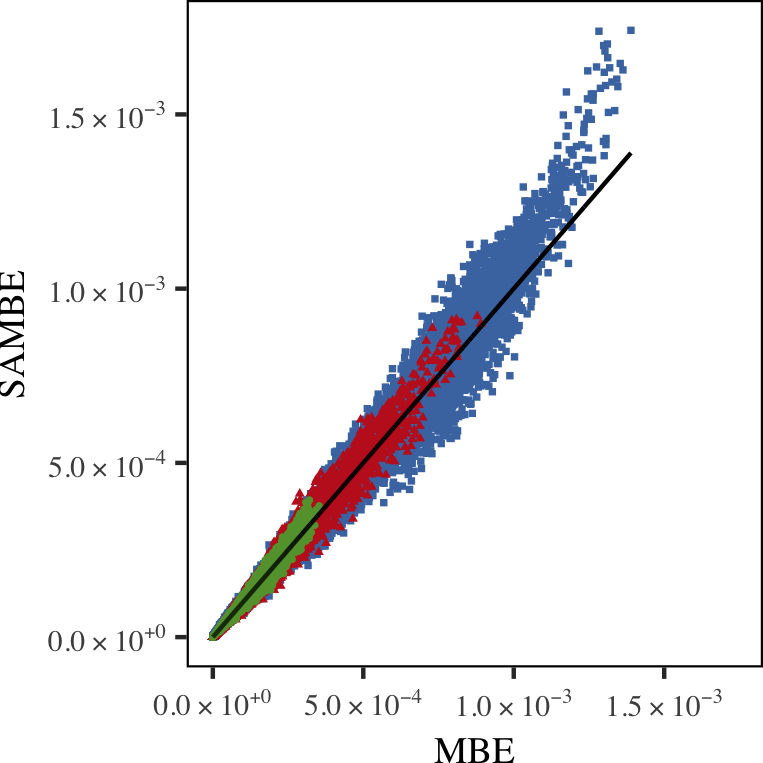
\includegraphics[keepaspectratio=true, width=\textwidth, height=0.23\textheight]{discussion/img/ferdosi_2_60000_mbe_sambe.png}
		\caption{Dataset \ferdosiTwo}
		\label{fig:discussion:multisphere:mbevssambe:ferdosi2}
	\end{subfigure}
	\begin{subfigure}{0.23\textwidth}
		\centering
		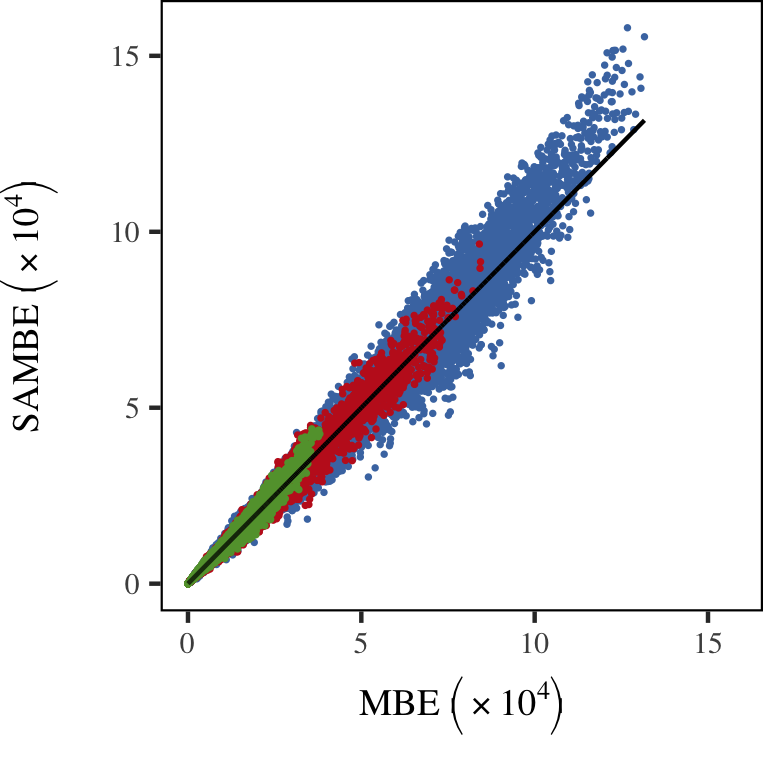
\includegraphics[keepaspectratio=true, width=\textwidth, height=0.23\textheight]{discussion/img/baakman_2_60000_mbe_sambe.png}
		\caption{Dataset \baakmanTwo}
		\label{fig:discussion:multisphere:mbevssambe:baakmanTwo}
	\end{subfigure}	
	\caption{Plots of the density estimated by \sambe as a function of those estimated by \mbe for dataset %
		\subref{fig:discussion:multisphere:mbevssambe:ferdosi2} % 
		\ferdosiTwo and %
		\subref{fig:discussion:multisphere:mbevssambe:baakmanTwo} %
		\baakmanTwo.
	}
	\label{fig:discussion:multisphere:mbevssambe}
\end{figure}

\begin{figure}
	\centering
	\begin{subfigure}{0.23\textwidth}
		\centering
		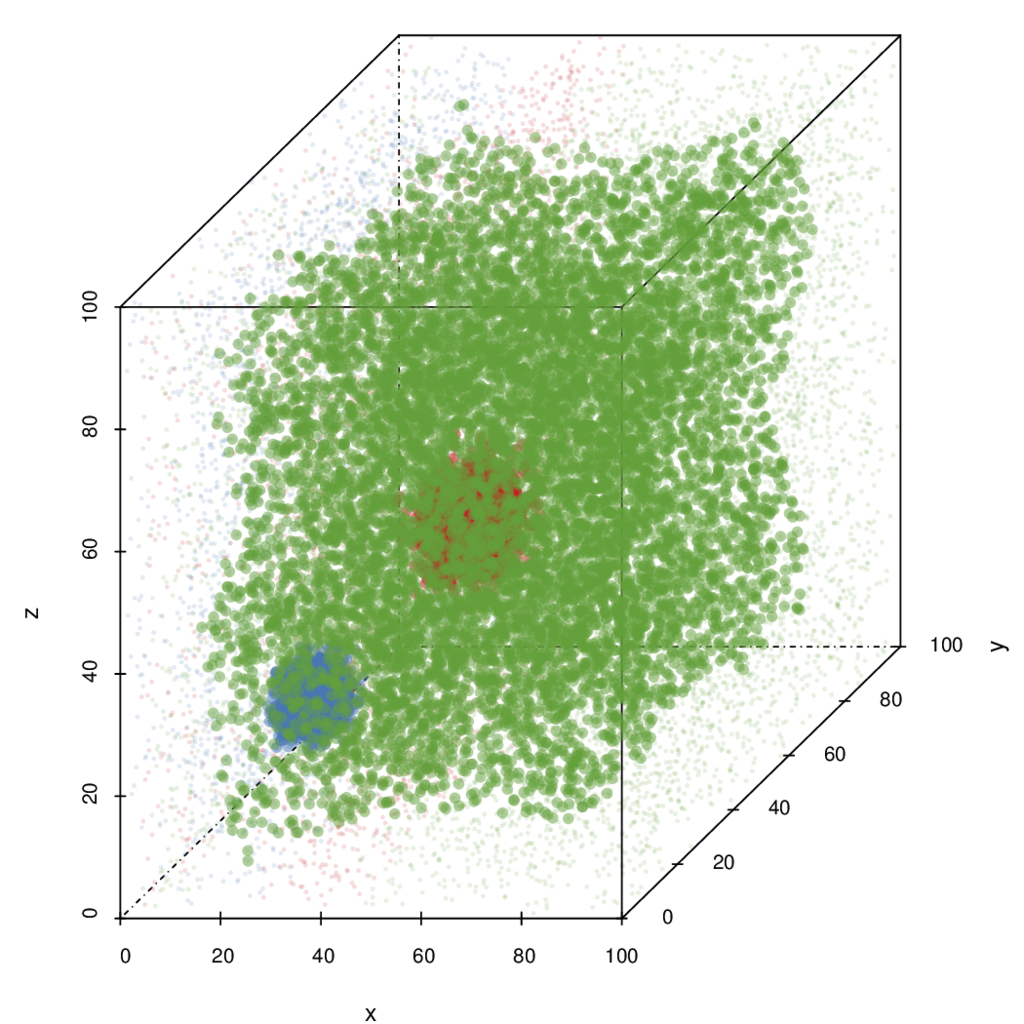
\includegraphics[keepaspectratio=true, width=\textwidth, height=0.23\textheight]{discussion/img/ferdosi_2_abs_error_mbeSmallerThansambe.pdf}
		\caption{Dataset \ferdosiTwo}
		\label{fig:discussion:multisphere:mbeLoweError:ferdosi2}
	\end{subfigure}
	\begin{subfigure}{0.23\textwidth}
		\centering
		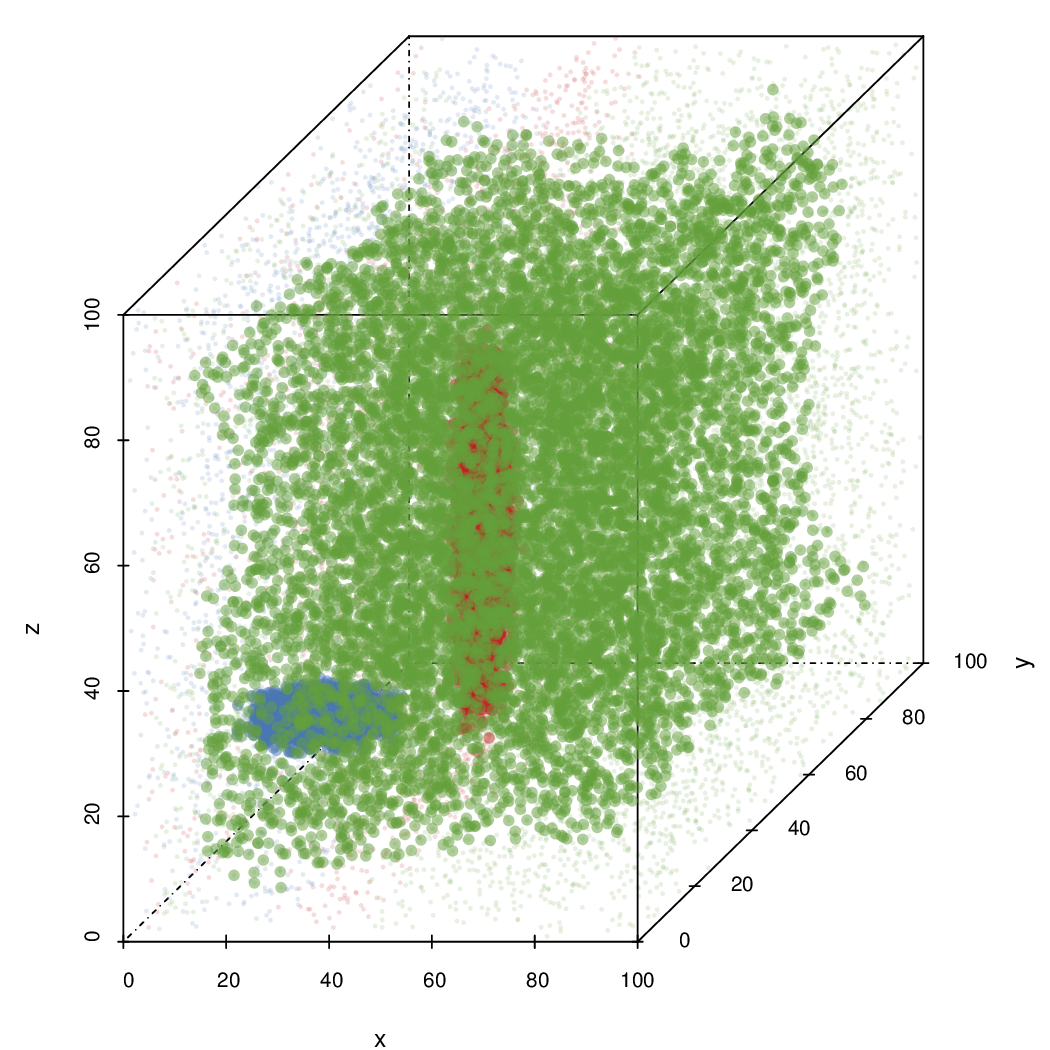
\includegraphics[keepaspectratio=true, width=\textwidth, height=0.23\textheight]{discussion/img/baakman_2_abs_error_mbeSmallerThansambe.pdf}
		\caption{Dataset \baakmanTwo}
		\label{fig:discussion:multisphere:mbeLoweError:baakmanTwo}
	\end{subfigure}	
	\caption{Low opacity scatter plot of the dataset with an overlay of high opacity larger points where the absolute error of \mbe is smaller than the absolute error of \sambe of %
		\subref{fig:discussion:multisphere:mbeLoweError:ferdosi2} % 
		\ferdosiTwo and %
		\subref{fig:discussion:multisphere:mbeLoweError:baakmanTwo} %
		\baakmanTwo.
	}
	\label{fig:discussion:multisphere:mbeLoweError}
\end{figure}


% Dataset Specific Questions
% Ferdosi 2 & Baakman 2
\todo[inline]{SAMBE zou visueel een kleinere error moeten hebben, maar gemiddeld komt MBE beter uit de bus? Op welke punten doet SAMBE het significiant beter / slechter dan MBE?}

% Ferdosi 3 & Baakman 3
\todo[inline]{Waarom is de error op baakman3 kleiner dan op ferdosi 3?}